\documentclass{article}
\usepackage{algpseudocode}%insert Algorithms
\usepackage[margin=1in]{geometry}
\usepackage{graphicx}%inorder to insert photo into article
\usepackage{algpseudocode}%algorithm package
\usepackage{hyperref}% including URLs
\usepackage{multirow}%for table
\usepackage{caption,subcaption}%we can import multiple packages within single usepackage
\usepackage{enumitem}
\title{}
\author{}
\date{}
\begin{document}
	\maketitle
	\section {introduction}
		Latex:Typesetting for professional documents latex isn't WISYWIG.
		WISYWIG:What you see is what you get.
		HTML: Hyper text Markup Language -> for Web Pages.
		XML:Extensible Markup Language Like: <first name> REX <first name> is tagged Between.
		Graph ML: Represents graph, edge and so on.
		Latex: not Wrapped, tags are not wrapped.
		Latex Focuses On Content.
		\subsection{Setting Up Latex}
			1.A TeX Distribution (type Setting Engine)
			2.A LaTeX editor
			\subsubsection{.log}
				.log contains every thing in console and etc
	\section{Word Faces}
		We can make \textbf{Bold} or \emph{italic} or \underline{Underline} our Words.
		if we don't want indent our preceding paragraph we use \textbf{no indent} command like as is. \noindent{}
	\section{Environment}
		\subsection{Bulleted Lists}
			C Based Programming Languages:
			\begin{itemize}
				\item C++
				\item C
				\item C\#%We use \ before Special Characters
			\end{itemize}
		\subsection{Numbered Lists}
			Materials you need to start Programming:
			\begin{enumerate}
				\item PC
				\item Internet Access
				\item Encourage
			\end{enumerate}
		\subsection{Description}
			We use this mode to describe items:
			\begin{description}
				\item[Python] Python is a interpretable Language.
				\item[C \& C++] Are Compiler Based Languages.
				\item[Java] Uses Both Interpretation and Compilation Benefits With \emph{JVM}.
			\end{description}
		\subsection{White Spaces}
			LaTeX ignores White Spaces \& Indentations in Code. So far So No Problem.
	\section{Tabular Environment}
 		ASCII Table In different formats \\\\ %\\ starts new line
		\begin{tabular}{lll|l}%for | sign Press: Shift + \ keys
			Dec & Hex & bin & Character\\
			\hline
			0 & 0 & 0 & \emph{[NULL]}\\
			1 & 1 & 1 & \emph{[START OF HEADING]}\\
		\end{tabular}
		\\ \\ \\
		\begin{tabular}{|lll|l|}
			\hline
			Dec & Hex & bin & Character\\
			\hline
			2 & 2 & 10 & \emph{[START OF TEXT]}\\
			3 & 3 & 11 & \emph{[END OF TEXT]}\\
			\hline
		\end{tabular}
		\\ \\ \\
		\begin{tabular}{|crl||c|} %c:center r:right l:left
			\hline
			Dec & Hex & bin & Character\\
			\hline \hline
			4 & 4 & 100 & \emph{[END OF TRANSMISSION]}\\
			5 & 5 & 101 & \emph{[ENQUIRY]}\\
			\hline
		\end{tabular}
	\\ \\
		Table is is a floating environment and we can Wrap tabular environments into tables \LaTeX Will Find Best Place to Place table And Also we can Apply Our Preferences.
		\\For Example We Wrapped Following Table in an \emph{Environment}:\\
		\begin{table}[htbp]%Priority From left to right h:Here t:Top b:Bottom p:Next Page
			\begin{center}
				\begin{tabular}{|lll|l|}
					\hline
					Dec & Hex & bin & Character\\
					\hline
					6 & 6 & 110 & \emph{[ACKNOWLEDGE]}\\
					% Methodes Below Are used to create Space between Table Sections
					%\bigskip
					%\smallskip
					\vspace{1cm}
					7 & 7 & 111 & \emph{[BELL]}\\
					127 & 7F & 1111111 & \emph{[DEL]}\\
					\hline
				\end{tabular}
			\end{center}
			\caption{Part Of ASCII Table}
			\label{tab:ASCII} %Labeling inorder to use in Other Places By: ~\ref{tab:ASCII}
		\end{table}
			\subsection{Recommendation}
				Always Use Tabular Environments.
			\subsection{Spanning Tables}
				\begin{table}[htp]
					\caption{Spanning rows and columns}
					\begin{center}
						\begin{tabular}{|l|c|c|}
							\hline
							&\multicolumn{2}{c|}{Ranges}\\
							&X&Y\\
							\hline
							\multirow{2}{*}{hot}&7&9\\%* means natural width
							&5&8\\
							&6&7\\
							\hline
							\multirow{3}{*}{cold}&4&7\\
							&2&9\\&3&5\\
							\hline
						\end{tabular}
					\end{center}
					\label{tab:multi}
				\end{table}
	\section{Photo}
		In order to use photo in \LaTeX Documents we must import \emph{graphicx} library using \textbf{usepakage}\\ \\
		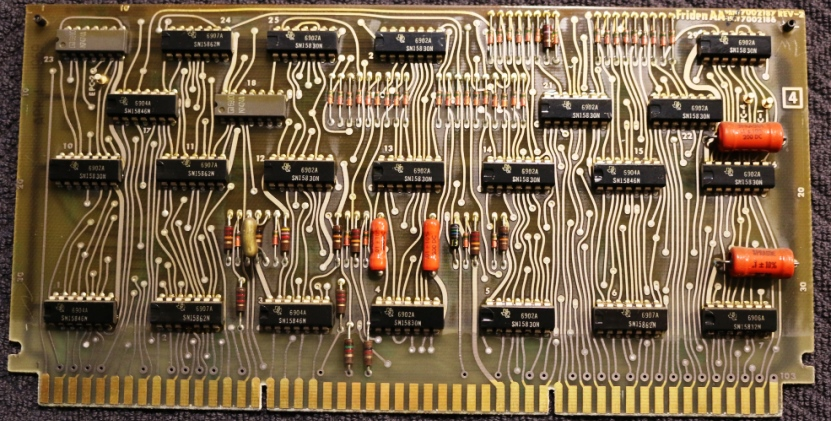
\includegraphics[width=3in]{f1160-board4-l.jpg}
		%Environment for photo
		\begin{figure}[htbp]
			\begin{center}
				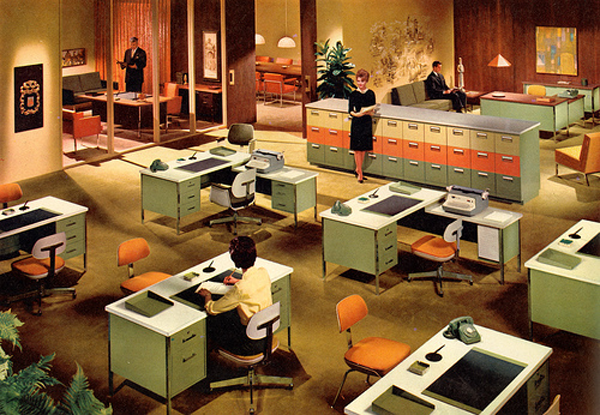
\includegraphics[width=4in]{desks.png}
				\caption{This is a office environment in 80s}
				\label{fig:Office}
			\end{center}
		\end{figure}
	\section{Article}

		We can cite Article or Books in our latex file. first of all we collect our citations in \emph{.bib} file and in \LaTeX file we cite them.for example ~\cite{smit54} is a book and ~\cite{LaTeX} is file.\\
		When we import references from \emph{.bib} file,\LaTeX Enumerate them in Automatic manner and \emph{.bbl} file will be created for further usages.
		\subsection{Reference Manager Software}
			Bibliothek and Mendeley are commonly used soft-wares that are used for create and export \emph{.bib} files.
	\section{Mathematics}
		\subsection{Equations}
			like $E=mc^2$ We can type many Equations inline Using \$ sign.\\
			Floating Environments Also Suggested for Mathematical Equation like  Mentioned in ~\ref{eq:simpEq} .
			\begin{equation}
				I=A^{-1}*A
				\label{eq:simpEq}
			\end{equation}
		\subsection{Special Characters}
			There are lots of special characters in mathematics that are also recognized by latex. some of them are mentioned below.
			\begin{equation}
				7^4+6*17\geq  13\cup X\alpha 13\exists \rightarrow \beta \cup \sigma
			\end{equation}
	\section{Algorithm}
		Algorithm Environment!
		\begin{algorithmic}
			\Procedure{Dec-MDP}{S,A,P,R,O,$\Omega$}\\
				\If{$ S \geq A$}\\
					$S \leftarrow A$ 
				\EndIf
			\EndProcedure
		\end{algorithmic}
	\section{Clickable Links}
		you can visit CTAN Website for more help:\url{https://ctan.org}
		\subsection{Article Template}
			you can use various journals templates. for example IEEE template :\url{http://www.ieee.org/publications_standards/publications/authors/author_templates.html} downloaded wile may have \emph{.bst} file for bibliography typesetting. Using Downloaded template:\\
			\textbackslash documentclass[conference]\{IEEEtran\}
	\section{More Photos}
		This photo of paper that ~\ref{fig:paper} and Figure ~\ref{fig:page} in figure ~\ref{fig:subs}.
		\begin{figure}[htp]
			\begin{center}
				\begin{subfigure}[b]{0.2\textwidth}
					\centering%instead of center Environment
					
\includegraphics[scale=0.8]{paper.jpeg}
					\caption{Beginning}\label{fig:paper}
				\end{subfigure}
				\\
				\begin{subfigure}[b]{0.2\textwidth}
					\centering
					
\includegraphics[scale=0.7]{page.png}
					\caption{End}
					\label{fig:page}
				\end{subfigure}
				\caption{The Process}
				\label{fig:subs}
			\end{center}
		\end{figure}
	\section{Parallel Cooperation in \LaTeX}
		when we importing specific file in our destination \LaTeX file ,for example this \LaTeX file we must import that using \textbackslash input\{file name within same folder without \emph{.tex} Extension\}.\\
		In source file any additional doesn't necessary.
	\section{Solving Enumeration Problem}
		Some times we start Enumerating For Example say Countries we end up with problems:
		\begin{enumerate}
			\item America
			\item Canada
			\item Brazil
		\end{enumerate}
		Then We explain some thing \& we enumerate again:
		\begin{enumerate}
			\item Japan
			\item China
		\end{enumerate}
		\subsection{First Solution}
			it will reset the counter after explanation between.\\
			Importing \emph{enumitem} will solve this problem. so we can use resume as parameter for enumeration environment \textbf{EXCEPT} first Environment.
			\begin{enumerate}
				\item America
				\item Canada
				\item Brazil
			\end{enumerate}
			Then We explain some thing \& we enumerate again:
			\begin{enumerate}[resume]
				\item Japan
				\item China
			\end{enumerate}
	\section{conclusion}
		Use \LaTeX \, you Microsoft Slave!
	\section{References}
	\bibliographystyle{plain}
	\bibliography{SAMPLE}% importing .bib file without mentioning .bib extension
\end{document}
